\documentclass{article}

\usepackage{arxiv}

\usepackage[utf8]{inputenc} % allow utf-8 input
\usepackage[T1]{fontenc}    % use 8-bit T1 fonts
\usepackage{hyperref}       % hyperlinks
\usepackage{url}            % simple URL typesetting
\usepackage{booktabs}       % professional-quality tables
\usepackage{amsfonts}       % blackboard math symbols
\usepackage{nicefrac}       % compact symbols for 1/2, etc.
\usepackage{microtype}      % microtypography
\usepackage{lipsum}
\usepackage{graphicx}

\title{Nested 3D neural networks for kidney and tumor segmentation}


\author{
  Olmo Zavala-Romero,\\
  %\thanks{Use footnote for providing further webpage, alternative address)---\emph{not} for acknowledging funding agencies.} \\
  Department of Radiation Oncology\\
  Sylvester Comprehensive Cancer Center, University of Miami\\
  1475 NW 12th Avenue Miami, FL 33136\\
  \texttt{osz1@miami.edu} \\
  %% examples of more authors
  \And
  Javier \\
  \texttt{} \\
  \AND
  Ignacio Alvarez Illan,\\
  Signal Theory and Communications Department\\
  Universidad de Granada, 18071 Granada, Spain\\
  \texttt{illan@ugr.es} \\
  \AND
  Radka Stoyanova\\
  Department of Radiation Oncology\\
  Sylvester Comprehensive Cancer Center, University of Miami\\
  1475 NW 12th Avenue Miami, FL 33136\\
  \texttt{rstoyanova@med.miami.edu} \\
  \AND
 Adrian L. Breto\\
 Department of Radiation Oncology\\
 Sylvester Comprehensive Cancer Center, University of Miami\\
 1475 NW 12th Avenue
 Miami, FL 33136\\
 \texttt{a.breto@umiami.edu} \\
 \AND
  Jorge Zavala-Hidalgo\\
  Centro de Ciencias de la Atm\'osfera\\
  Universidad Nacional Aut\'onoma de M\'exico, Mexico City, M'exico\\
  \texttt{jzavala@atmosfera.unam.mx} \\
  \AND
  Rosario Romero-Centeno\\
  Centro de Ciencias de la Atm\'osfera\\
  Universidad Nacional Aut\'onoma de M\'exico, Mexico City, M\'exico\\
  \texttt{rosario@atmosfera.unam.mx} \\
}

\begin{document}
\maketitle

\begin{abstract}

\end{abstract}


% keywords can be removed
\keywords{First keyword \and Second keyword \and More}

\section{Introduction}
\label{sec:intro}

Kidney cancer has an high number of diagnosed cases each year, being invasive techniques the most common treatment\cite{sun_treatment_2012}. Machine learning techniques have been proven to provide valuable tools in medical imaging, increasing the accuracy in diagnosis for several diseases\cite{erickson_machine_2017}. In recent years, deep learning techniques have increased the performance of classical machine learning approaches in several imaging problems, including medical image analysis\cite{litjens_survey_2017}. In this work, we propose a deep learning approach for kidney cancer detection and segmentation, as participants of the Kits19 challenge.

\section{Methodology}
\label{sec:methods}
\subsection{Data}

The data used in this study belongs to the Kits19 challenge\cite{heller_kits19_2019}, which consists of 544 patients who underwent radical nephrectomy of partial nephrectomy, reviewed at the University of Minnesota, with a selection of 300 patients that met the inclusion criteria. These patients have annotated CT abdominal images, with two annotations: kidneys and tumors. The data was separated in training and testing data, and the annotations where only available in the 210 patients training set to the challenge participants. 

\label{sec:data}
\subsection{Preprocessing}
\label{sec:prepro}
The proprocessing steps performed are:
\begin{enumerate}
    \item Resample the image to a resolution of $2 \times 2 \times 2$ mm. 
    \item Crop a cube of size $168^3$ from the center of the image. 
    \item Normalize the intensities to a range of 0 to 1.
\end{enumerate}

\subsection{Neural Network Architecture}
\label{sec:nnarc}
The proposed method contains two NN with the same architecture, one is used to segment the kidneys and the other one 
is used to segment the tumors. 

Each NN is a 3D U-Net with 14 convolutional layers. Each convolutional layer uses relu as the activation function and
all the filters are of size of $3\times 3 \times 3$. The input size is the preprocessed image with size $168^3$. 
Last layer is sigmoid.
Uses SGD for the optimization method, and batch normalization to improve the generalization. 
% TODO stop mechanism, loss equations. 
The loss function is negative DSC.
For the tumor the loss function only takes into account the values inside the predicted kindey. 

\begin{figure}[h]
    \centering
    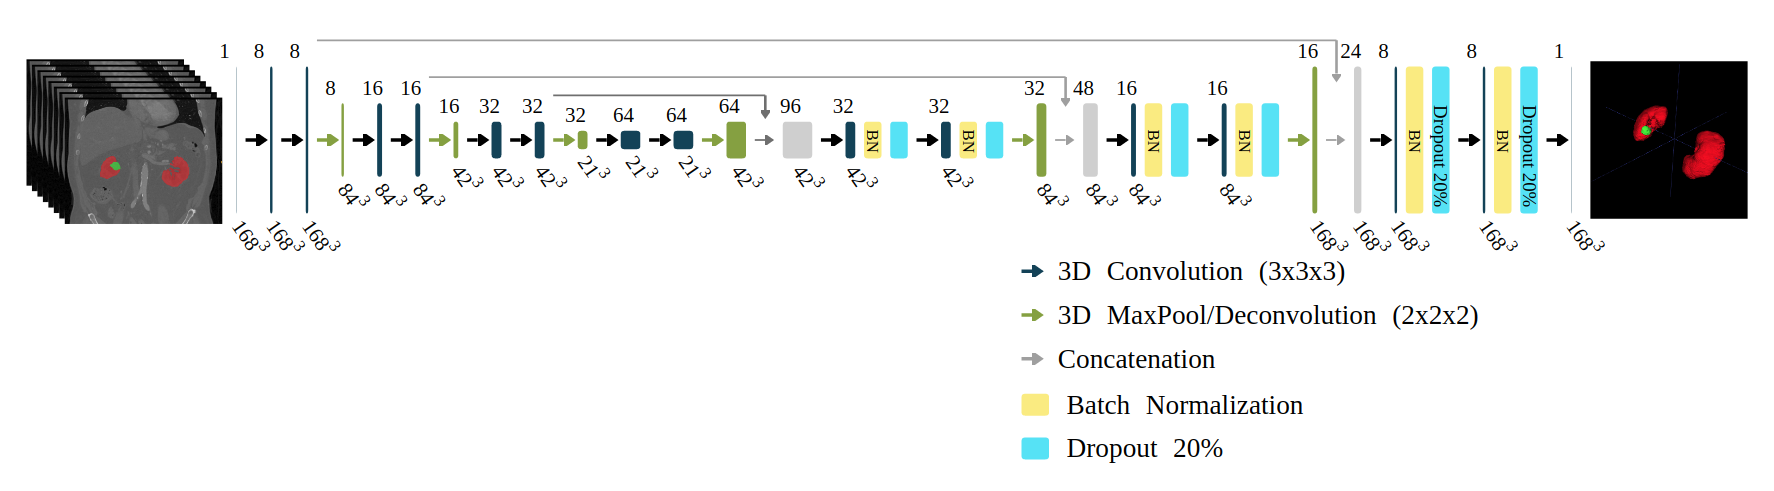
\includegraphics[totalheight=.20\textheight]{imgs/nn.png}
    \caption{NN architecture }
    \label{fig:mobile1}
\end{figure}

\bibliography{references}

\end{document}
